% main.tex
\documentclass{article}

\usepackage[pdfauthor={CoderDojo Linz},
            pdftitle={Feuerwerk in TypeScript}]
            {hyperref}



\newcommand{\footertitle}{Bubble sorter in Scratch}
% settings.tex
\usepackage[
    a4paper, 
    top=2cm,
    left=1cm,
    right=1cm,
    bottom=2cm
]{geometry}

\usepackage{fontspec}
\usepackage{graphicx}
\usepackage{hyperref}
\usepackage{fancyhdr}
\usepackage[ngerman]{babel}
\usepackage{wrapfig}
\usepackage{enumitem}
\usepackage{titlesec} 
\usepackage{ragged2e}
\usepackage{tcolorbox}
\usepackage{array}
\usepackage[table]{xcolor}
\usepackage{fontawesome5}

\setmainfont{Carlito}

% Fancyhdr setup
\fancypagestyle{defaultpagestyle}{
    \fancyhf{} % Clear all headers and footers
    \fancyhead[C]{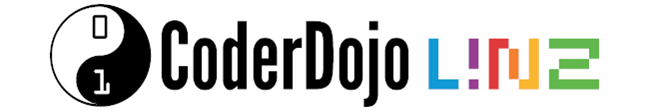
\includegraphics[width=5cm]{../../CoderDojo_Logo.png}} 
    \renewcommand{\headrulewidth}{0pt} % Remove header line
    \renewcommand{\footrulewidth}{0pt} % Remove footer line
    \fancyfoot[L]{\footertitle}
    \fancyfoot[R]{Seite \thepage} % Right footer with page number
}

\newcommand{\SectionDesign}[4]{
    \noindent
    \csname #1*\endcsname{\textcolor[HTML]{1E90FF}{\fontsize{#2pt}{#3pt}\selectfont #4}}
}

\newcommand{\TextAndImage}[5][{}]{
    \fontsize{11pt}{16pt}\selectfont
    \noindent
    \begin{minipage}[c]{#4\textwidth}
    \RaggedRight
    #2 % First parameter: text
    \end{minipage}
    \hfill
    \begin{minipage}[c]{#5\textwidth}
    \includegraphics[width=\textwidth, #1]{#3} % Second parameter: image file name
    \end{minipage}
}

\newcommand{\ImageAndText}[2]{
    \fontsize{16pt}{24pt}\selectfont
    \noindent
    \begin{minipage}[c]{0.65\textwidth}
        \includegraphics[width=\textwidth]{#1} % Second parameter: image file name
    \end{minipage}
    \hfill % Fills the space between the minipages
    \begin{minipage}[c]{0.25\textwidth}
        \centering
        #2 % First parameter: text
    \end{minipage}
}

\newcommand{\TextDesign}[1]{
    \fontsize{11pt}{16pt}\selectfont
    \noindent
    \RaggedRight
    #1 % First parameter: text
}
\graphicspath{{images/}}

\begin{document}
    \pagestyle{defaultpagestyle}

    \SectionDesign{section}{24}{24}{\textbf{Bubble Sorter mit Scratch}}
    \vspace{1cm}
     
    \ImageAndText{MainPic.png}{
    \centering
    Heute programmieren wir eine herausfordernde Scratch Übung namens Bubble Sorter. Hierbei kannst du deine Scratch Kenntnisse verbessern.
    }{0.6}{0.3}{16}{24}
    
    \vspace{2cm}
    \SectionDesign{subsection}{18}{24}{\textbf{Ziel der Übung}}
    \vspace{0.5cm}

    \TextDesign{
    Heute wollen wir gemeinsam einen Bubble Sorter basteln, hierbei geht es darum den Algorithmus zu verstehen, mit Klonen zu Arbeiten und dich selber etwas heraus zu fordern.

    \vspace{\baselineskip}
    Du solltest für diese Übung schon ein wenig Programmiererfahrung mit einer Block programmiersprache wie \textit{Scratch} oder \textit{Snap!} haben. 
    }

    \vspace{1cm}
    \SectionDesign{subsection}{18}{24}{\textbf{Start}}
    \vspace{0.5cm}

    \TextDesign{
    Du brauchst für diese Übung keine spezielle Software auf deinem Computer zu installieren. Scratch kannst du auch im Web-browser verwenden. Um los zu legen müssen wir als erstes unsere Figuren und den Hintergrund fest legen. Wir brauchen dafür Bälle und natürlich ein Gefäß für unsere Bälle. Eine Figur die mit dem Benutzer spricht und einen schönen Hintergrund. In den Unteren Links kannst du dir deine Figuren runter laden}

\begin{itemize}
        \item \href{https://meet.coderdojo.net/biber-sprite}{Biber Figur}
        \item \href{https://meet.coderdojo.net/ball-sprite}{Ball Figur}
        \item \href{https://meet.coderdojo.net/behälter-sprite}{Behälter Figur}
    \end{itemize}
    
     % NEWPAGE
    \newpage
    
    \vspace{0.5cm}
    
    \SectionDesign{subsection}{18}{24}{\textbf{Hintergrund festlegen und zuschneiden}}
    \vspace{1cm}
     
    \ImageAndText{HintergrundBild.png}{
    
  Das hier wird der Hintergrund für unser Spiel ich werde dir gleich Zeigen wie man ihn einbindet in Scratch. 
    }{0.4}{0.3}{12}{24}
    
\vspace{1cm}
    \TextDesign{
    Als erstes schauen wir uns dafür unseren Start Bildschirm an wenn wir ein neues Projekt anlegen. Wenn du noch nichts verändert hast und deine Sprache auf Deutsch eingestellt ist sollte dein Start Bildschirm so aussehen: 
    } 
    \vspace{0.5cm}
    
    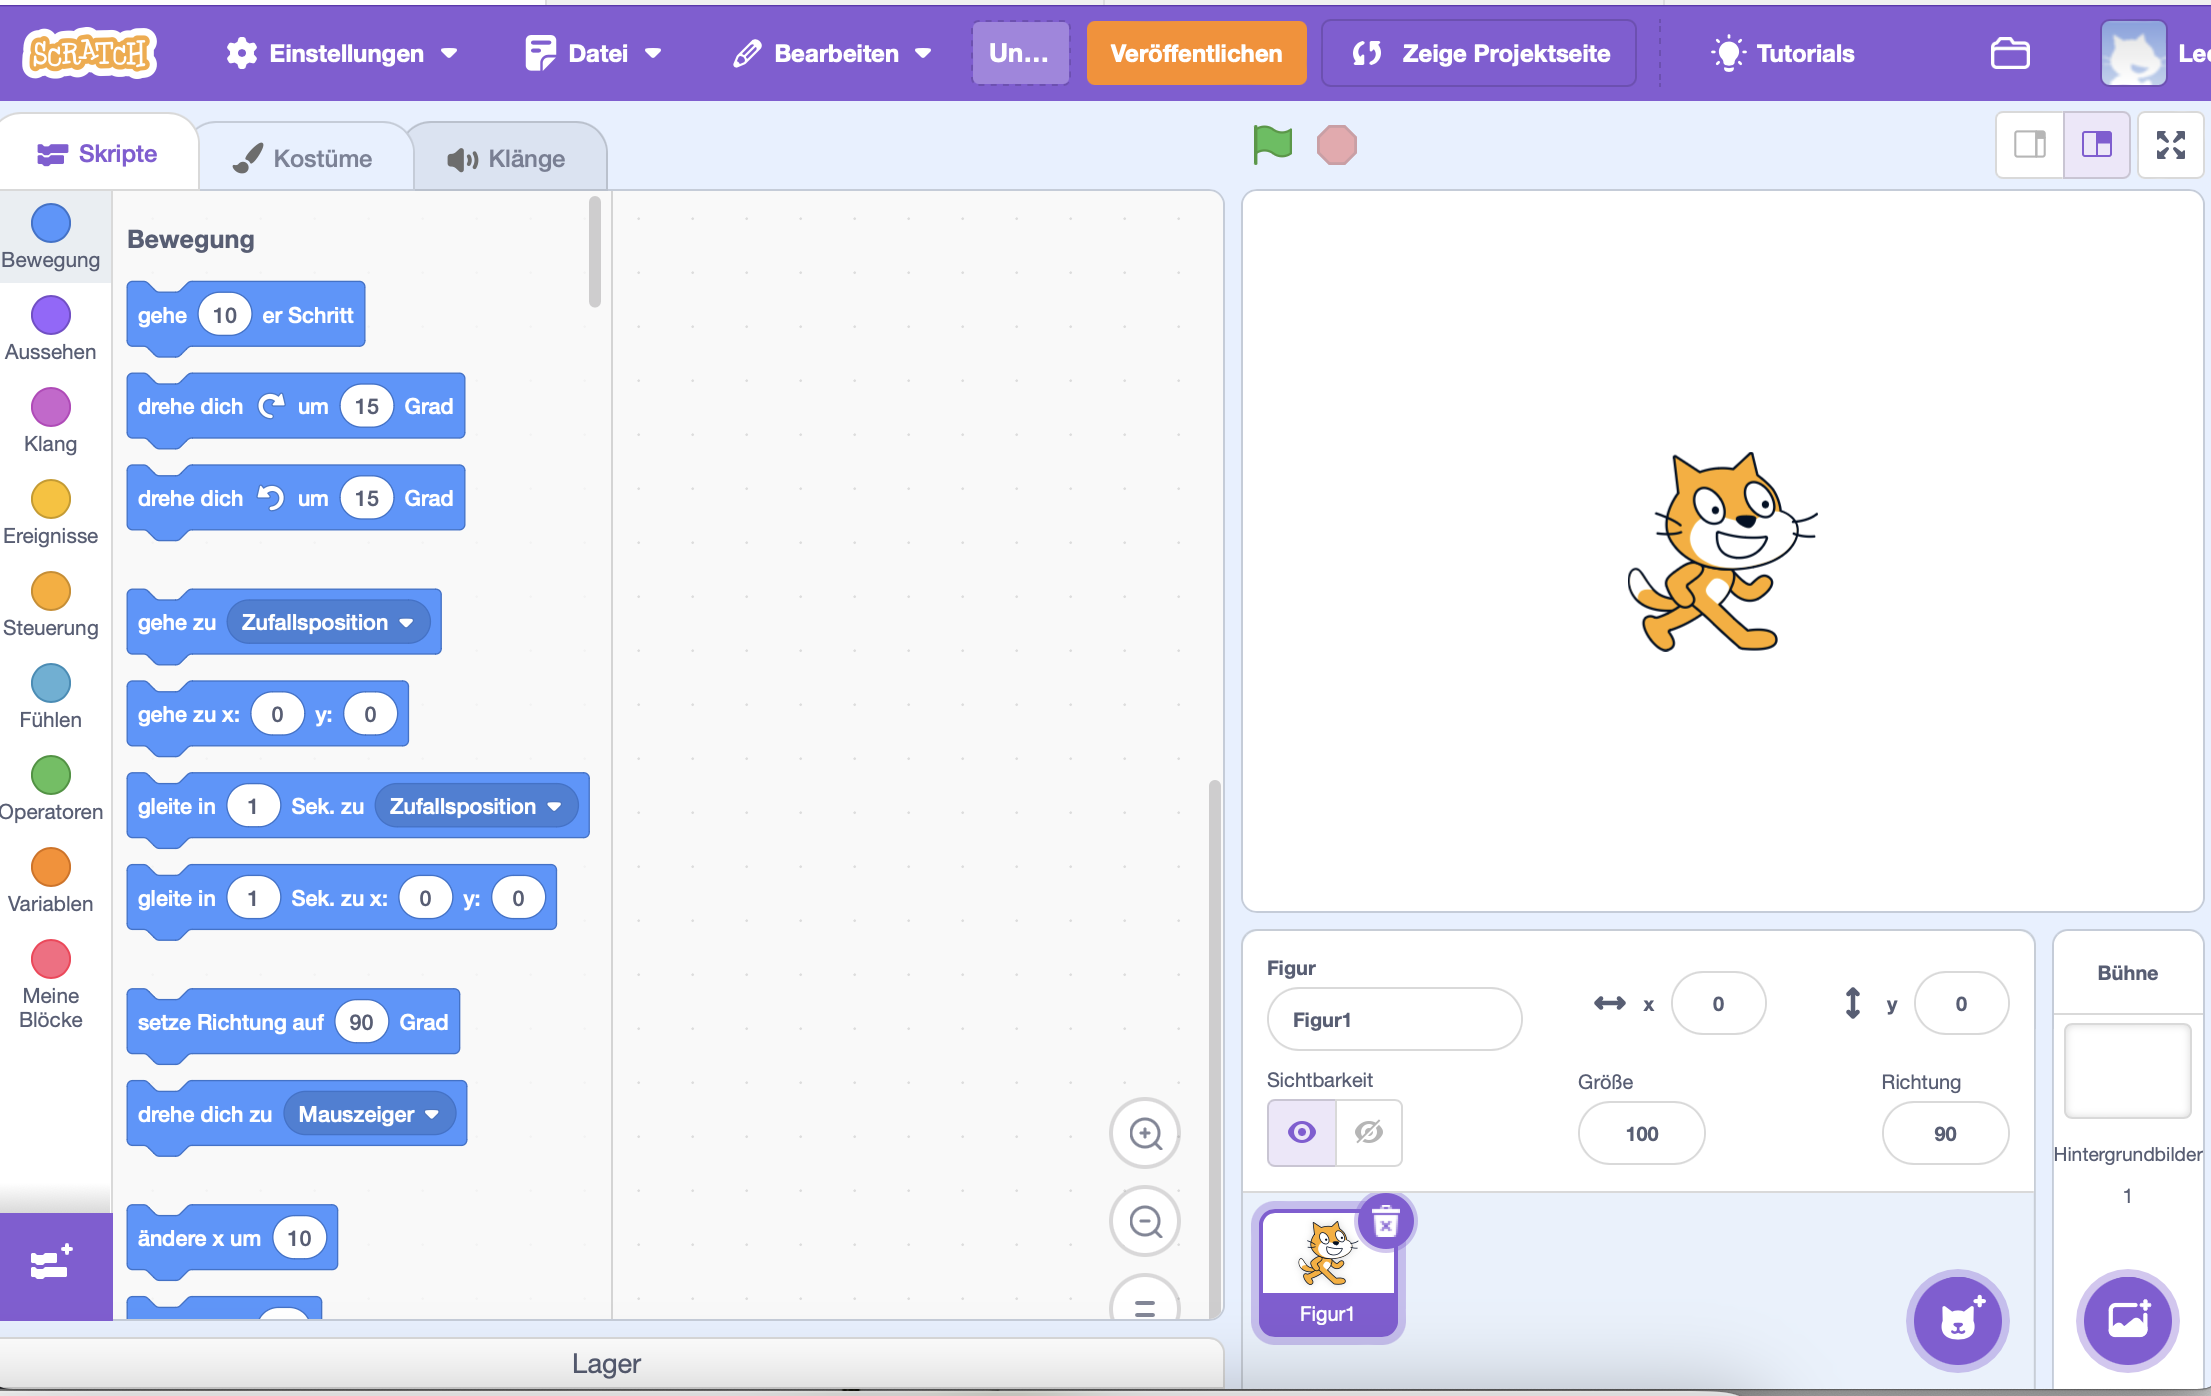
\includegraphics[width=0.5\textwidth, height=5cm]{Startbildschirm.png}

\vspace{0.5cm}

\TextAndImage{
    Wenn du auf das grüne Zeichen ganz unten auf der rechten Seite deines Bildschirmes klickst solltest du dieses Menü sehen. Um unseren eigenen Hintergrund hinzu zu fügen müssen wir ihn als erstes hochladen. Das machen wir mit den ganz obersten Zeichen (das mit dem Pfeil). Wenn du drauf klickst öffnen sich automatisch deine Dateien jetzt musst du nur noch das richtige Bild auswählen und "Hochladen" klicken.
}{HintergrundEinfügen.png}{0.4}{0.5}{11}{16}

\vspace{1cm}
    \TextDesign{
    Jetzt sollte dein Bildschirm automatisch so aussehen:
    } 
    \vspace{0.4cm}

    \includegraphics[width=0.5\textwidth, height=5cm]{StartbildschirmHZ.png}
    \vspace{1cm}

    
    \TextDesign{
    Wenn du dir die Vorschau (das kleinere rechte Bild) genauer ansiehst wirst du merken das wir oben und unten einen weißen Rand haben. Das wollen wir natürlich nicht deshalb müssen wir das Bild zurecht schneiden. Links auf deinen Bildschirm kannst du dein Hintergrund Bild bearbeiten. Hier siehst du das aktuell lila Zeichen mit dem Pfeil. Wenn du drauf klickst kannst du Sachen ausschneiden und dann vergrößern oder verkleinern. Klicke einmal auf das Zeichen und dann klicke mit deiner Maus (oder Mausped) auf die Linke obere Ecke und halte die Maus Taste, hier wirst du sehen das jetzt ein strichliertes Viereck entsteht wenn du den Zeiger bewegst. Ziehe deshalb deinen Zeiger an die rechte unter Ecke so das das ganze Bild markiert ist. 
    }
  \vspace{0.5cm}
    
       \ImageAndText{Zurechtschneiden.png}{
  Wenn es jetzt so aussieht hast es richtig gemacht und kannst es jetzt an den blauen ecken vergrößern bis kein weißer Rand mehr da ist. Du kannst es natürlich auch mit den oberen und unteren Punkten vergrößern und verkleinern dadurch verziehst du aber das Bild. 
    }{0.4}{0.5}{12}{24}
    


\vspace{0.5cm}


\SectionDesign{subsection}{18}{24}{\textbf{Gefäße}}

\vspace{0.5cm}

\TextAndImage{
   Wir fangen an mit unseren Gefäßen für die Bälle. Der erste Block gibt nur an das das alles ausgeführt werden soll wenn die Fahne angeklickt wird. Der zweite lila Block ist dafür da das die Gefäße nicht vor den Bällen sind und sie verdecken. Mit den zwei blauen Blöcken werden x und y festgelegt das die Figur immer am Anfang genau auf der Position ist und man sie nicht beliebig verschieben kann. Hier haben wir in Orange eine Variable diese Sätzen wir auf null das unser erster Behälter auf der Position bleibt wo er ist. Danach klonen wir den Behälter 2 mal weil wir insgesamt drei Behälter haben wollen hier ändern wir auch die Position um 1 damit die nächsten Behälter nicht die gleiche Position wie der erste haben. Darunter haben wir noch einen kleinen Block dieser wird ausgeführt wenn der Klone erstellt wird und gibt ihm mit der Formel den richtigen Platz. Diese kannst du einfach nachbauen. 
    }{CupBlöcke.png}{0.5}{0.5}{11}{16}

    
    \newpage
    \vspace{0.5cm}
    
    \SectionDesign{subsection}{18}{24}{\textbf{Eigene Blöcke anlegen}}

   
    \vspace{0.5cm}

    \TextAndImage{
  Du wirst ganz viele eigene Blöcke in dieser Übung brauchen. Falls du nicht weist wie man Blöcke erstellt kommt hier eine Anleitung dazu ;) Wenn du in deiner Block Liste gaaannz nach unten gehst findest du einen roten Bereich mit neuer Block dort klickst du drauf. Mache unten bei "Ohne Bildschirmaktuallisierung laufen lassen" ein Häkchen hin. Wir werden bei dieser Übung erstmals auch nur zusätzlich Eingabefelder dazu brauchen diese kannst du mit den Lila markierten Knopf hinzu fügen. Übrigens die Einteilung in Blöcken strukturiert das Programm in Textueller Programmierung wird das mit Methoden, Klassen und Funktionen gemacht. Ein großer Vorteil davon ist das man Blöcke immer wider verwenden kann wo man sonst vielleicht den gleichen Code zweimal brauchen würde.
    }{NeuenBlockErstellen.png}{0.4}{0.4}{11}{16}

    \vspace{0.5cm}
\SectionDesign{subsection}{18}{24}{\textbf{Erste Blöcke }}

          \vspace{0.5cm}

 \TextAndImage{
In diesen Block fragen wir den Benutzer in welchen Behälter er den Ball tun möchte. Du kannst ihn mal nachbauen und schauen was raus kommt! Probier ruhig alles mögliche ein zu geben fällt dir was auf? 
    }{ZielGefäß1.png}{0.4}{0.4}{11}{16}
    
    \vspace{0.5cm}

     \TextAndImage{
Falls du den Fehler nicht gefunden hast ist es nicht schlimm. Wir dürfen naetürlich wie bei unseren ersten Block nur Zahlen zwischen 1 und 3 eingeben weil wir in unseren Fall nur 3 Behälter haben. Das machen wir mit einen "Falls" Block. Probiere dich jetzt wider durch und überlege was noch schief gehen könnte! 
    }{ZielGefäß2.png}{0.4}{0.4}{11}{16}

        \vspace{0.5cm}

     \TextAndImage{
Richtig! Falls du den Fehler nicht gefunden hast ist das auch nicht schlimm! Wir müssen natürlich schauen ob die Farbe darunter stimmt das machen wir ebenfalls wider mit einen "Falls" Block. Einen Fehler haben wir noch. Kleiner Tipp: Überlege in welchen Behälter wir Kugeln hinzu fügen können! 
    }{ZielGefäß3.png}{0.4}{0.6}{11}{16}


           \vspace{0.5cm}

     \TextAndImage{
Genau! wir müssen natürlich noch prüfen ob der Behälter nicht mehr als 3 Kugeln beinhaltet ist! Eine Schleife brauchen wir Zusätzlich das wir immer wider fragen wenn etwas nicht zutrifft das wird ganz einfach mit der Variable "zu" gelöst. SUPER! dein zweiter Block ist fertig!
    }{ZielGefäß4.png}{0.4}{0.6}{11}{16}

    
 \vspace{0.5cm}

     \TextAndImage{
Als erstes fangen wir damit an den Benutzer zu fragen von wo er den Block überhaupt nehmen möchte. Du findest auf den Bildern auch immer Kommentare was dir den Block nochmals erklären. Das machen wir hier mit einer Frage und einer Variable worin wir die Antwort speichern. Probiere es doch mal aus. Findest du den Fehler?
    }{FrageQuell1.png}{0.4}{0.4}{11}{16}

     \vspace{0.5cm}

     
     \TextAndImage{
Richtig! Falls du den Fehler nicht gefunden hast ist das nicht schlimm! Wir dürfen natürlich nur Zahlen zwischen 1 und 3 eingeben weil wir in diesen Fall nur 3 Behälter haben. Das überprüfen wir  mt einen "Falls" Block. Probiere und überlege wider findest du noch einen Fehler?
    }{FrageQuell2.png}{0.4}{0.4}{11}{16}


     \vspace{0.5cm}

     
     \TextAndImage{
Genau! Falls du den Fehler nicht gefunden hast ist das nicht schlimm! Wir können den Ball nicht aus einen leeren Behälter nehmen! Das überprüfen wir wider mit einen "Falls" Block. Eine Hürde gibt es aber noch!
    }{FrageQuell3.png}{0.4}{0.4}{11}{16}

         \vspace{0.5cm}

     
     \TextAndImage{
Super!! Du bist fertig ! mit deinen zweiten Block. Die schleife brauchen wir genau wie in den letzten Block das unser Benutzer immer wider gefragt wird. 
    }{FrageQuell4.png}{0.4}{0.4}{11}{16}
\end{document}